\setcounter{ex}{0}

% --- CÂU 1 ---
\begin{ex}
	Cho hàm số $y = f(x)$ liên tục trên $(-3; 3)$ có đồ thị như hình vẽ. Số điểm cực trị của hàm số trên khoảng $(-3; 3)$ là?
	\begin{center}
		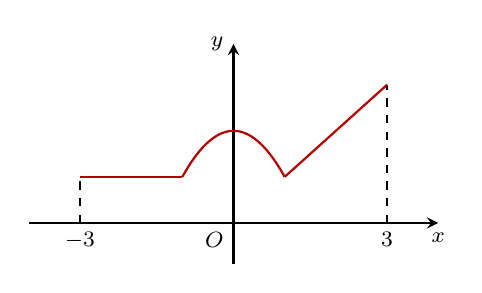
\begin{tikzpicture}[scale=0.65, font=\footnotesize, >=stealth]
			\draw[->, thick] (-4, 0) -- (4, 0) node[below] {$x$};
			\draw[->, thick] (0, -0.8) -- (0, 3.5) node[left] {$y$};
			\node[below left] at (0, 0) {$O$};
			\node[below] at (-3, 0) {$-3$};
			\node[below] at (3, 0) {$3$};
			\draw[dashed] (-3, 0) -- (-3, 0.9);
			\draw[dashed] (3, 0) -- (3, 2.7);
			\draw[thick, red!70!black] (-3, 0.9) -- (-1, 0.9);
			\draw[thick, red!70!black, smooth, samples=60, domain=-1:1] plot (\x, {1.8 - 0.9*(\x)^2});
			\draw[thick, red!70!black] (1, 0.9) -- (3, 2.7);
		\end{tikzpicture}
	\end{center}
	\shortans{2}
	\loigiai{
		Dựa vào đồ thị của hàm số $y = f(x)$ trên khoảng $(-3; 3)$:
		\begin{itemize}
			\item Trên khoảng $(-3; -1)$, hàm số không đổi (hằng số) nên không có điểm cực trị trên $(-3; -1]$.
			\item Tại điểm $x = 0$, đồ thị có điểm nhô lên cao nhất trong lân cận nên $x = 0$ là một điểm cực đại.
			\item Tại điểm $x = 1$, hàm số liên tục và đổi chiều từ nghịch biến sang đồng biến nên $x = 1$ là một điểm cực tiểu.
		\end{itemize}
		Vậy hàm số có $2$ điểm cực trị trên khoảng $(-3; 3)$.
	}
\end{ex}

% --- CÂU 2 ---
\begin{ex}
	Cho hàm số $f(x) = \dfrac{3x - m^2}{2x + 1}$, với $m$ là tham số. Tổng các giá trị của $m$ để $7\max_{[1; 3]} f(x) + 3\min_{[1; 3]} f(x) = 4$ bằng
	\shortans{0}
	\loigiai{
		Hàm số $f(x) = \dfrac{3x - m^2}{2x + 1}$ xác định và liên tục trên đoạn $[1; 3]$.\\
		Ta có $f'(x) = \dfrac{3 + 2m^2}{(2x + 1)^2} > 0, \forall x \in [1; 3]$ và $\forall m \in \mathbb{R}$.\\
		Do đó hàm số luôn đồng biến trên đoạn $[1; 3]$, suy ra:
		$$\min_{[1; 3]} f(x) = f(1) = \dfrac{3 - m^2}{3}, \quad \max_{[1; 3]} f(x) = f(3) = \dfrac{9 - m^2}{7}.$$
		Thay vào giả thiết bài toán:
		$$7\max_{[1; 3]} f(x) + 3\min_{[1; 3]} f(x) = 4 \iff 7\cdot\dfrac{9 - m^2}{7} + 3\cdot\dfrac{3 - m^2}{3} = 4 \iff (9 - m^2) + (3 - m^2) = 4$$
		$$\iff 12 - 2m^2 = 4 \iff m^2 = 4 \iff m = \pm 2.$$
		Vậy tổng các giá trị của $m$ là $(-2) + 2 = 0$.
	}
\end{ex}

% --- CÂU 3 ---
\begin{ex}
	Đồ thị của hàm số $y = f(x) = \dfrac{2x^3 + 9x^2 + 5}{x^2 + 2x + 2}$ có một tiệm cận xiên là đường thẳng $d$. Đường thẳng $d$ đi qua một điểm $M$ có tung độ bằng $2007$ thì hoành độ điểm $M$ là bao nhiêu?
	\shortans{1001}
	\loigiai{
		Thực hiện phép chia đa thức tử cho mẫu, ta có:
		$$y = \dfrac{2x^3 + 9x^2 + 5}{x^2 + 2x + 2} = 2x + 5 - \dfrac{14x + 5}{x^2 + 2x + 2}.$$
		Vì $\lim_{x \to \pm\infty} \left[y - (2x + 5)\right] = \lim_{x \to \pm\infty} \left(-\dfrac{14x + 5}{x^2 + 2x + 2}\right) = 0$ nên tiệm cận xiên của đồ thị hàm số là đường thẳng $d\colon y = 2x + 5$.\\
		Điểm $M(x_M; 2007) \in d$ nên:
		$$2x_M + 5 = 2007 \iff 2x_M = 2002 \iff x_M = 1001.$$
	}
\end{ex}

% --- CÂU 4 ---
\begin{ex}
	Một căn phòng dạng hình hộp chữ nhật với chiều dài $8\text{ m}$, rộng $6\text{ m}$ và cao $4\text{ m}$ có hai chiếc quạt treo tường. Chiếc quạt $A$ treo chính giữa bức tường $8\text{ m}$ và cách trần $1\text{ m}$, chiếc quạt $B$ treo chính giữa bức tường $6\text{ m}$ và cách trần $1{,}5\text{ m}$. Hỏi khoảng cách giữa hai chiếc quạt $A$ và $B$ cách nhau bao nhiêu $\text{m}$ (làm tròn đến hàng phần trăm)?
	\shortans{5,02}
	\loigiai{
		Chọn hệ trục tọa độ $Oxyz$ sao cho gốc $O$ tại một góc sàn nhà (giao của bức tường $8\text{ m}$ chứa quạt $A$ và bức tường $6\text{ m}$ chứa quạt $B$), tia $Ox$ dọc theo chiều dài $8\text{ m}$, tia $Oy$ dọc theo chiều rộng $6\text{ m}$ và tia $Oz$ hướng thẳng đứng lên trần nhà (cao $4\text{ m}$).
		\begin{itemize}
			\item Chiếc quạt $A$ nằm chính giữa bức tường $8\text{ m}$ (thuộc mặt phẳng $(Oxz)$) và cách trần $1\text{ m}$ nên có tọa độ: $A(4; 0; 4 - 1) = (4; 0; 3)$.
			\item Chiếc quạt $B$ nằm chính giữa bức tường $6\text{ m}$ (thuộc mặt phẳng $(Oyz)$) và cách trần $1{,}5\text{ m}$ nên có tọa độ: $B(0; 3; 4 - 1{,}5) = (0; 3; 2{,}5)$.
		\end{itemize}
		Khoảng cách giữa hai chiếc quạt $A$ và $B$ là:
		$$AB = \sqrt{(0 - 4)^2 + (3 - 0)^2 + (2{,}5 - 3)^2} = \sqrt{16 + 9 + 0{,}25} = \sqrt{25{,}25} \approx 5{,}02\text{ (m)}.$$
	}
\end{ex}

% --- CÂU 5 ---
\begin{ex}
	Một sợi dây kim loại dài $60\text{ cm}$ được cắt thành hai đoạn. Đoạn thứ nhất được uốn thành một hình vuông, đoạn thứ hai được uốn thành một vòng tròn. Hỏi khi tổng diện tích của hình vuông và hình tròn ở trên nhỏ nhất thì chiều dài đoạn dây uốn thành hình vuông bằng bao nhiêu (làm tròn đến hàng phần chục)?
	\shortans{33,6}
	\loigiai{
		Gọi $x\text{ (cm)}$ là chiều dài đoạn dây uốn thành hình vuông ($0 < x < 60$). Khi đó chiều dài đoạn dây uốn thành vòng tròn là $60 - x\text{ (cm)}$.
		\begin{itemize}
			\item Hình vuông có chu vi $x$ nên độ dài cạnh là $\dfrac{x}{4}$ và diện tích là $S_1 = \left(\dfrac{x}{4}\right)^2 = \dfrac{x^2}{16}$.
			\item Hình tròn có chu vi $60 - x$ nên bán kính là $R = \dfrac{60 - x}{2\pi}$ và diện tích là $S_2 = \pi R^2 = \dfrac{(60 - x)^2}{4\pi}$.
		\end{itemize}
		Tổng diện tích của hình vuông và hình tròn là:
		$$S(x) = \dfrac{x^2}{16} + \dfrac{(60 - x)^2}{4\pi}, \quad x \in (0; 60).$$
		Ta có đạo hàm:
		$$S'(x) = \dfrac{x}{8} - \dfrac{60 - x}{2\pi} = 0 \iff \pi x = 4(60 - x) \iff (\pi + 4)x = 240 \iff x = \dfrac{240}{\pi + 4} \approx 33{,}6\text{ (cm)}.$$
		Vì $S''(x) = \dfrac{1}{8} + \dfrac{1}{2\pi} > 0$ nên $S(x)$ đạt giá trị nhỏ nhất tại $x \approx 33{,}6\text{ cm}$.
	}
\end{ex}

% --- CÂU 6 ---
\begin{ex}
	Để làm một máng xối nước có dạng hình lăng trụ, từ một tấm tôn kích thước $0{,}75\text{ m} \times 4\text{ m}$ người ta gấp tấm tôn đó như hình vẽ dưới. Biết mặt cắt của máng xối (được cắt bởi mặt phẳng song song với hai đầu máng xối) là một hình thang cân có đáy nhỏ và hai cạnh bên đều bằng $0{,}25\text{ m}$; còn đáy lớn có độ dài bằng $x\text{ (m)}$. Tìm thể tích lớn nhất máng xối được tạo thành? (kết quả làm tròn đến hàng phần trăm theo đơn vị $\text{m}^3$).
	\begin{center}
		\begin{tikzpicture}[scale=0.95, font=\footnotesize, >=stealth]
			% (a) Tấm tôn
			\begin{scope}[xshift=0cm]
				\draw[thick] (0, 0) rectangle (3.2, 1.8);
				\node[above] at (1.6, 1.8) {$4\text{ m}$};
				\node[left] at (0, 0.9) {$0{,}75\text{ m}$};
				\node[below] at (1.6, -0.3) {(a) Tấm tôn};
			\end{scope}
			% (b) Máng xối
			\begin{scope}[xshift=4.3cm, yshift=0.2cm]
				\coordinate (A) at (0, 1.0);
				\coordinate (B) at (0.6, 0.2);
				\coordinate (C) at (1.4, 0.0);
				\coordinate (D) at (2.2, 0.5);
				\coordinate (v) at (1.6, 0.8);
				\coordinate (A') at ($(A)+(v)$);
				\coordinate (B') at ($(B)+(v)$);
				\coordinate (C') at ($(C)+(v)$);
				\coordinate (D') at ($(D)+(v)$);
				\draw[thick] (A) -- (B) -- (C) -- (D) -- cycle;
				\draw[thick] (A) -- (A') -- (D') -- (D);
				\draw[thick] (C) -- (C') -- (D');
				\draw[dashed] (B) -- (B');
				\draw[dashed] (A') -- (B') -- (C');
				\draw[dashed] (A') -- ($(B')!0.5!(C')$) node[midway, right] {$0{,}25\text{ m}$};
				\node[below left] at (1.0, 0.1) {$4\text{ m}$};
				\node[below right] at (2.2, 0.0) {$0{,}25\text{ m}$};
				\node[below] at (1.9, -0.5) {(b) Máng xối};
			\end{scope}
			% (c) Mặt cắt
			\begin{scope}[xshift=8.8cm, yshift=0.3cm]
				\draw[thick] (0, 1.3) -- (0.7, 0) -- (2.1, 0) -- (2.8, 1.3) -- cycle;
				\node[above] at (1.4, 1.3) {$x\text{ (m)}$};
				\node[below] at (1.4, 0) {$0{,}25\text{ m}$};
				\node[left] at (0.35, 0.65) {$0{,}25\text{ m}$};
				\node[right] at (2.45, 0.65) {$0{,}25\text{ m}$};
				\node[below] at (1.4, -0.6) {(c) Mặt cắt};
			\end{scope}
		\end{tikzpicture}
	\end{center}
	\shortans{0,32}
	\loigiai{
		Mặt cắt là hình thang cân có đáy nhỏ $a = 0{,}25 = \dfrac{1}{4}\text{ (m)}$, hai cạnh bên bằng $\dfrac{1}{4}\text{ (m)}$ và đáy lớn $x\text{ (m)}$ với $\dfrac{1}{4} < x < \dfrac{3}{4}$.\\
		Chiều cao của hình thang cân mặt cắt là:
		$$h = \sqrt{\left(\dfrac{1}{4}\right)^2 - \left(\dfrac{x - \dfrac{1}{4}}{2}\right)^2} = \dfrac{1}{2}\sqrt{\dfrac{1}{4} - \left(x - \dfrac{1}{4}\right)^2}.$$
		Diện tích mặt cắt ngang của máng xối là:
		$$S(x) = \dfrac{x + \dfrac{1}{4}}{2} \cdot h = \dfrac{1}{4}\left(x + \dfrac{1}{4}\right)\sqrt{\dfrac{1}{4} - \left(x - \dfrac{1}{4}\right)^2}.$$
		Đặt $t = x - \dfrac{1}{4} \in \left(0; \dfrac{1}{4}\right)$, khi đó $x + \dfrac{1}{4} = t + \dfrac{1}{2}$ và:
		$$S(t) = \dfrac{1}{4}\left(t + \dfrac{1}{2}\right)\sqrt{\dfrac{1}{4} - t^2}.$$
		Ta có:
		$$S'(t) = \dfrac{1}{4}\cdot\dfrac{\dfrac{1}{4} - \dfrac{1}{2}t - 2t^2}{\sqrt{\dfrac{1}{4} - t^2}} = 0 \iff 2t^2 + \dfrac{1}{2}t - \dfrac{1}{4} = 0 \iff t = \dfrac{1}{4}\text{ (do } t > 0\text{)}.$$
		Khi $t = \dfrac{1}{4}$ (tức $x = 0{,}5\text{ m}$), diện tích mặt cắt đạt giá trị lớn nhất là:
		$$S_{\max} = \dfrac{1}{4}\cdot\left(\dfrac{1}{4} + \dfrac{1}{2}\right)\sqrt{\dfrac{1}{4} - \dfrac{1}{16}} = \dfrac{3\sqrt{3}}{64}\text{ (m}^2\text{)}.$$
		Thể tích lớn nhất của máng xối (chiều dài $l = 4\text{ m}$) là:
		$$V_{\max} = 4 \cdot S_{\max} = 4 \cdot \dfrac{3\sqrt{3}}{64} = \dfrac{3\sqrt{3}}{16} \approx 0{,}3248 \approx 0{,}32\text{ (m}^3\text{)}.$$
	}
\end{ex}
